\documentclass[11pt, a4paper]{article}
\usepackage[spanish]{babel}
\usepackage{graphicx}
\usepackage{amssymb}
\usepackage{enumerate}
\title{\bf{Cuadril\'ateros c\'iclicos - La perspectiva general}}
\author{Yufei Zhao}
\date{}
\begin{document}
	\maketitle
	Una habilidad importante de cualquier ol\'impico geom\'etra es la capacidad de reconocer configuraciones notables.
	
	De hecho, muchos problemas de geometr\'ia son constru\'idos basados en algunos temas comunes. En esta lectura, exploraremos una de estas configuraciones.
	\section{¿Qu\'e tienen en com\'un estos problemas?}
	\begin{enumerate}
	\item (IMO 1985) Un c\'irculo con centro O pasa atrav\'es de los v\'ertices $A$ y $C$ del tri\'angulo $ABC$ e interseca a los segmentos $AB$ y $BC$ en los puntos $K$ y $N$, respectivamente. Los circunc\'irculos de los tri\'angulos $ABC$ y $KBN$ se intersecan exactamente en dos puntos distintos $B$ y $M$. Probar que $\angle OMB = 90^{\circ}$
	\begin{figure}[h]
		\centering
		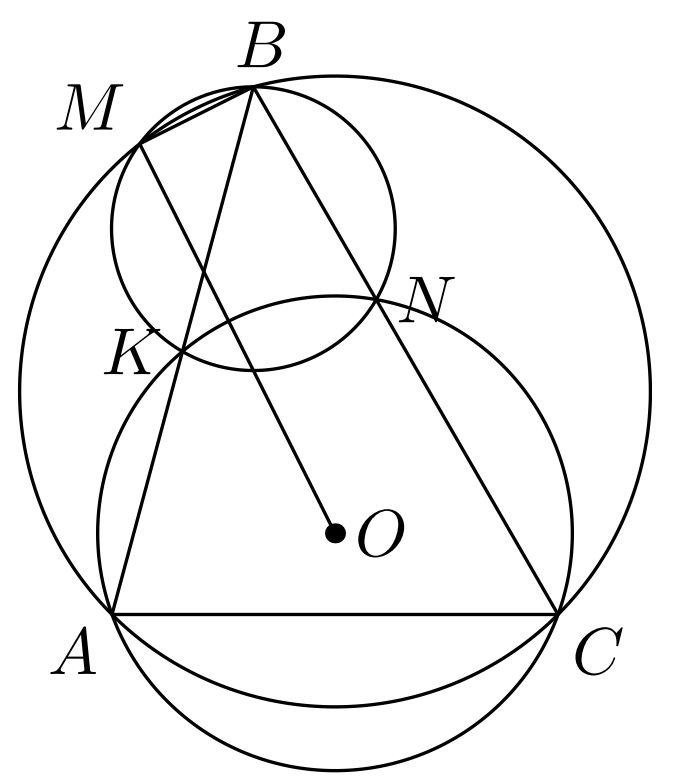
\includegraphics[scale=0.18]{p1.1x}
	\end{figure}
	\item (Rusia 1995; TST de Rumania 1996; Iran 1997) Sea un c\'irculo de di\'ametro $AB$ y centro $O$, y sean $C$ y $D$ dos puntos de este c\'irculo. La l\'inea $CD$ interseca a la l\'inea $AB$ en el punto $M$ satisfaciendo $MB < MA$ y $MD < MC$. Sea $K$ el punto de intersecci\'on (distinto de O) de los circunc\'irculos de los tri\'angulos $AOC$ y $DOB$. Demuestra que $\angle MKO = 90^{\circ}$
		\newpage
	\begin{figure}[h!]
		\centering
		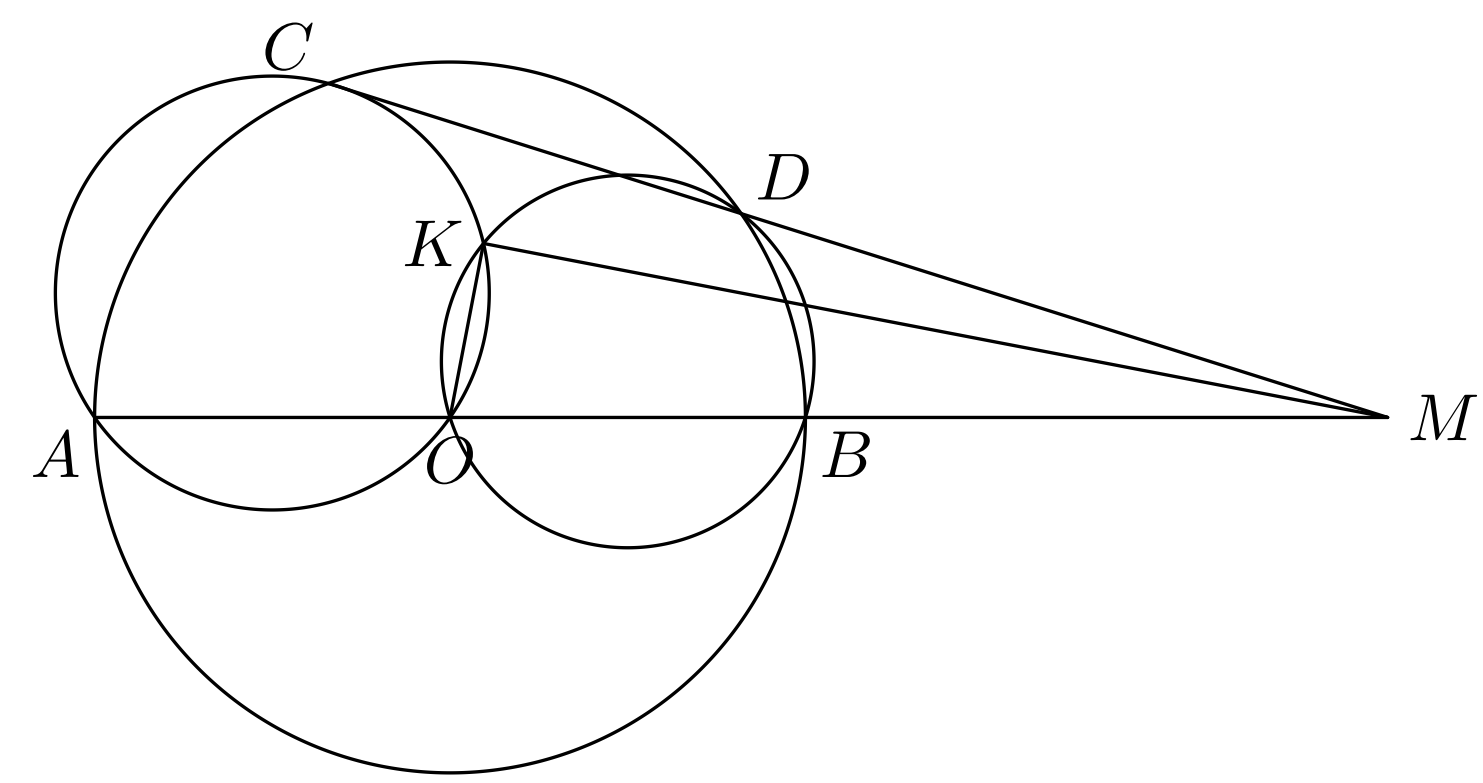
\includegraphics[scale=0.18]{p1.2}
	\end{figure}
	\item (USA TST 2007) El tri\'angulo $ABC$ est\'a inscrito en el c\'irculo $\omega$. Las l\'ineas tangentes a $\omega$ en $B$ y $C$ se intersecan en el punto $T$. El punto $S$ se encuentra en el rayo $BC$ tal que $AS \perp AT$. Los puntos $B_1$ y $C_1$ est\'an en el rayo $ST$ ($C_1$ est\'a entre $B_1$ y $S$) Tal que $B_1T = BT = C_1T$. Probar que los tri\'angulos $ABC$ y $AB_1C_1$ son proporcionales entre s\'i.
	\begin{figure}[h]
		\centering
		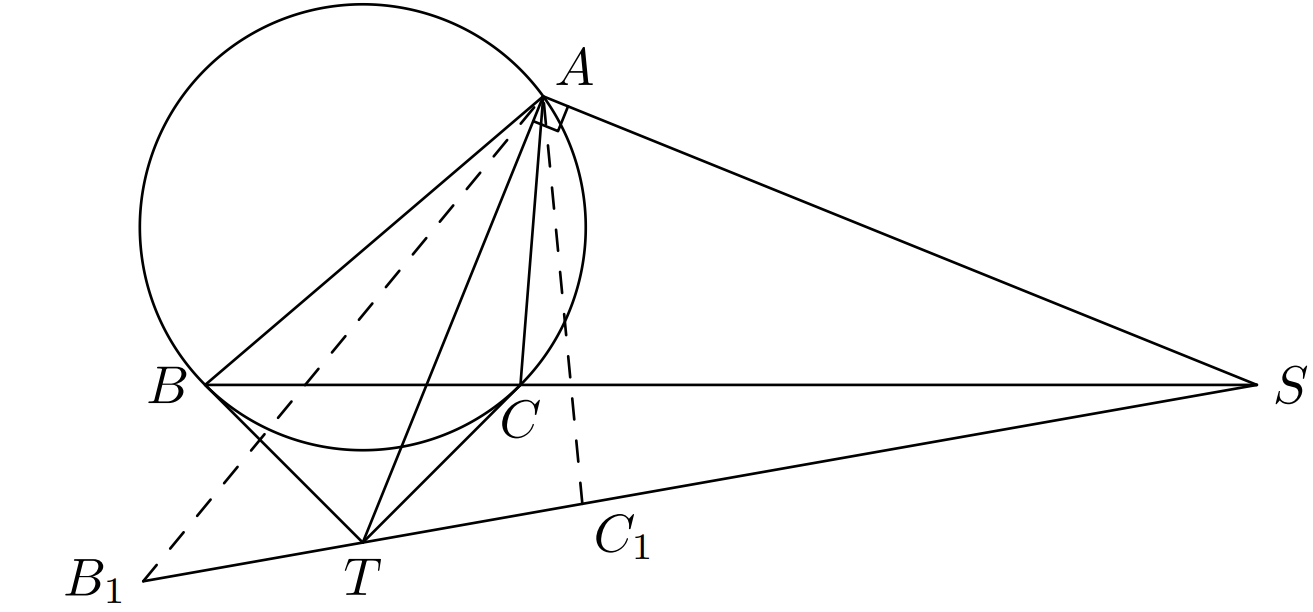
\includegraphics[scale=0.2]{p1.3}
	\end{figure}
	Aunque estas configuraciones geom\'etricas parecen muy diferentes a primera vista, en realidad est\'an muy relacionadas. De hecho, son solo pedazitos de un gran diagrama!
\newpage
\section{Un Gran Diagrama}
\begin{figure}[h]
	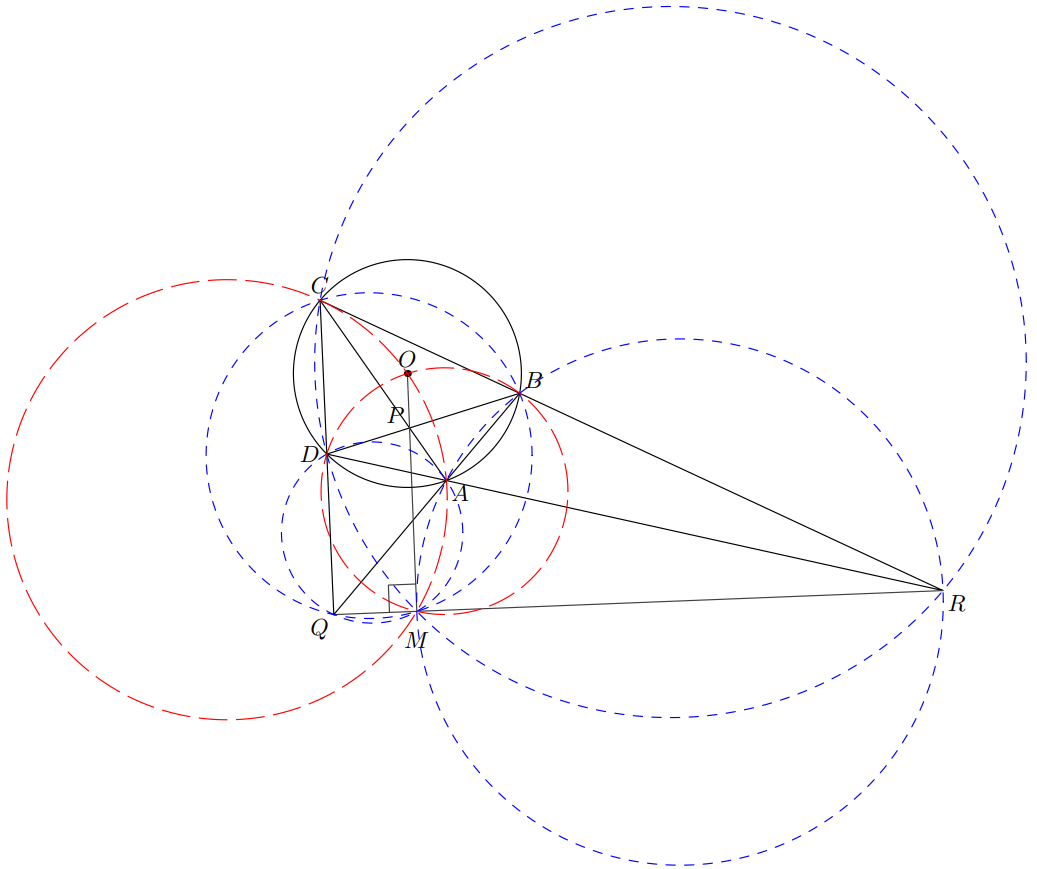
\includegraphics[scale=0.5]{fig1}
	\centering
	\caption{La perspectiva general}
\end{figure}
En esta lecci\'on, trataremos de entender las propiedades de la Figura 1. Hay muchas cosas ocurriendo en este di\'agrama y al verlo puede ser aterrador, pero no te preocupes, lo superaremos paso a paso. En el proceso, discutiremos algunas t\'ecnicas geom\'etricas que tambi\'en son \'utiles en otros lugares.
(¿Puedes decir d\'onde podemos encontrar cada uno de los problemas de la Secci\'on 1 en la Figura 1? Probablemente no puedas hacerlo ahora mismo, pero ojala seas capaz al final de esta clase)
\section{Teoeorema de Miquel y el punto de Miquel}
\textbf{Hecho 1.} (El teorema de Miquel) Sea $ABC$ un triangulo, y sean $X, Y, Z$ puntos en las l\'ineas $BC, CA, AB$, respectivamente. Asume que los seis puntos $A, B, C, X, Y, Z$ son todos distintos. Luego, los circunc\'irculos de $AYZ, BZX, CXY$ pasan a trav\'es de un punto en com\'un.
\begin{figure}[h]
	\centering
	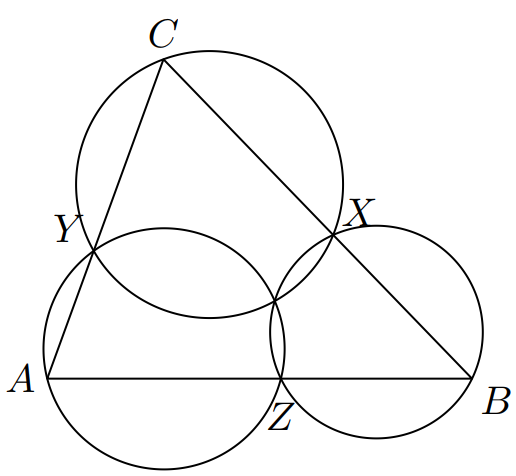
\includegraphics[scale=0.3]{p3.1}
	\caption{Diagrama para el Hecho (Teorema de Miquel)}
\end{figure}
\end{enumerate}
\textbf{Ejercicio 1.} Probar el punto 1.(Es muy f\'acil solo busca\footnote{Si te molestan los problemas de configuraci\'on y orientaci\'on (Y deber\'ia!), usa \'angulos dirigidos} a algunos \'angulos)\\

\textbf{Hecho 2} (Punto de Miquel) Sean $\ell_1, \ell_2, \ell_3, \ell_4$ cuatro l\'ineas en el plano, donde ninguna es paralela entre s\'i. Utilicemos $C_{ijk}$ para denotar el circunc\'irculo de los tri\'angulos formados por las l\'ineas $\ell_i, \ell_j, \ell_k$ (Estos c\'irculos son llamados c\'irculos de Miquel). Luego $C_{123}, C_{124}, C_{134}, C_{234}$ pasan a trav\'es de un punto en com\'un (llamado el Punto de Miquel)\\

\textbf{Ejercicio 2.} Probar el punto 2 (Pista: Aplicar el teorema 1) \\

Queremos enfocarnos en el caso de cuadril\'atero c\'iclico.
\begin{figure}[h]
	\centering
	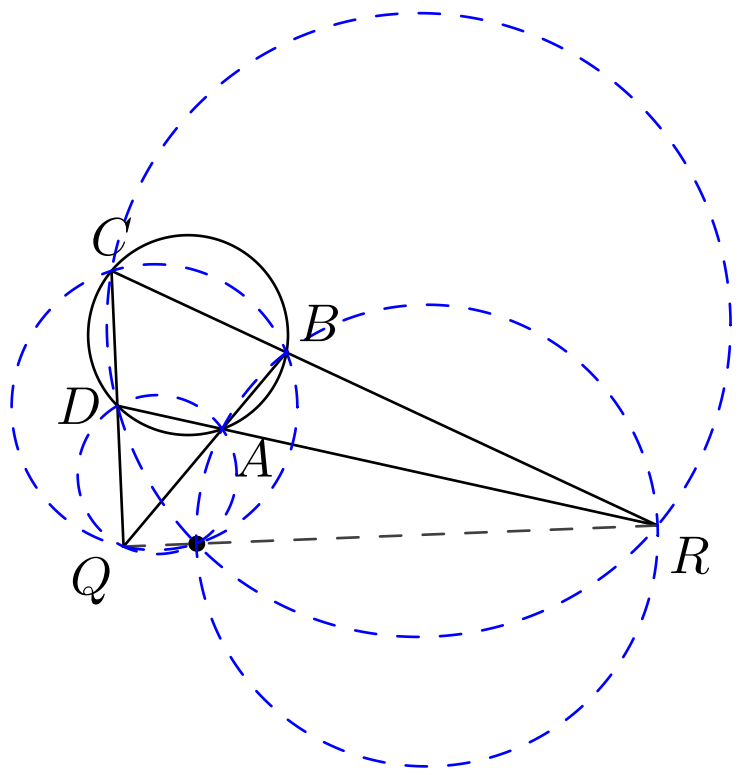
\includegraphics[scale=0.25]{p3.2}
	\caption{Punto de Miquel para el cuadril\'atero c\'iclico $ABCD$}
\end{figure}
\textbf{Hecho 3.} Sea $ABCD$ un cuadril\'atero. Las rectas $AB$ y $CD$ chocan en $Q$, y las rectas $DA$ y $CB$ chocan en $R$. Luego el punto de Miquel de $ABCD$ (i.e El segundo punto de intersecci\'on de $ADQ$ y $ABR$) est\'a en la recta $QR$ si y solo si $ABCD$ es c\'iclico.\\

\textbf{Ejercicio 3.} Probar el Hecho 3 (Esto de nuevo es una f\'acil persecuci\'on de \'angulos)
\end{document}